The aim of this procedure is the estimation of the median spectral acceleration value $\hat{s}_c$, that brings the structure to the attainment of a set of damage states, and the corresponding dispersion beta $\beta_{sc}$, the parameters needed for the mathematical representation of fragility in equation \ref{eq:fragility-definition}. The aim is achieved making use of a R-$\mu$-T relationship, between the reduction factor R, the ductility $\mu$ and period T, which is based on the work of Dolsek and Fajfar (2004). The R-$\mu$-T-based procedure presented herein is applicable to any kind of multi-linear capacity curve, and it is suitable for single building fragility curve estimation, as described in section \ref{subsubsec:single-building-DF}. However the fragility curves derived for single buildings can be combined in a unique fragility curve, which considers the inter-building uncertainty, as described in section \ref{subsubsec:multiple-building-DF}.

\subsubsection{Single Building Fragility and Vulnerability function}
\label{subsubsec:single-building-DF}
The spectral value at each damage state threshold ds $\hat{S}_{a,ds}$ is found from the top displacement representing that ds attainment $\hat{\delta}_{roof, ds}$, as explained in C$_{R}$\_based procedure and reported the following equation:

\begin{equation}
\hat{S}_{a,ds}(T_1) = \frac{4 \pi^2}{\hat{C}_R T^2 \Gamma_1 \Phi_1} \hat{\delta}_{roof, ds}
\label{eq:basic_DF}
\end{equation}

The value of C$_R$, the ratio between the inelastic and the elastic spectral displacement, is found from equation \ref{eq:Cr_DF}.

\begin{equation}
\hat{C}_{R} = \frac{\mu_{LS}}{R_{LS}}
\label{eq:Cr_DF}
\end{equation}

where $\mu_{ds}$ and $R_{ds}$ are the ductility level and the reduction factor at each ds attainment. According to the results of an extensive parametric study using three different sets of recorded and semi-artificial ground motions Dolsek and Fajfar (2004) related the ductility demand, $\mu$ , and reduction factor, R , through the following formula:

\begin{equation}
\label{eq:mu_DF}
\mu = \frac{1}{c} (R-R_{0})+\mu_{0}
\end{equation}

In the proposed model, $\mu$ is linearly dependent on R within two reduction factor intervals. The parameter c defines the slope of the R–$\mu$ relation, and depends on the initial period of the system T, the ratio r$_{u}$, the reduction factor R and the corner periods T$_{c}$ and T$_{d}$. T$_{c}$ and T$_{d}$ are the corner periods between the constant acceleration and constant velocity part of the idealized elastic spectrum, and between the constant velocity and constant displacement part of the idealized elastic spectrum respectively.

Given the parameters of the multilinear pushover curves (R$_{\mu_{c}}$, $\mu_{c}$, r$_{u}$) and T, the median R-$\mu$ curve, similar to an IDA curve, can be construct using the aforementioned relationship.  A multilinear capacity curve and the corresponding R$_{\mu_{c}}$, $\mu_{c}$ and r$_{u}$ parameters are shown in Figure \ref{fig:quadrilinear_DF}.

\begin{figure}[H]
\centering
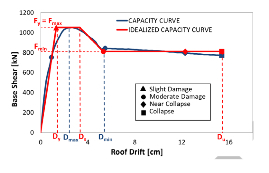
\includegraphics[width=10cm,height=5cm]{./figures/quadrilinearDF.jpg}
\caption{Multilinear capacity curve and parameters for the definition of R-$\mu$ relation.}
\label{fig:quadrilinear_DF}
\end{figure}

On the median "IDA curve" the $\mu$-R pairs corresponding to the limit states (R$_{LS}$ and $\mu_{LS}$) can be found and turned into median spectral acceleration values for that limit state $\hat{S}_c$, to be used in equation \ref{eq:basic_DF}.

Once median R$_{LS}$ and $\mu_{LS}$ are found, the 84 and 16 fractiles $\mu$ are extracted using top drift record-to-record dispersion $\sigma_{ln(\delta)}$ from equation \ref{eq:beta_eq_RGM}, by Ruiz-Garcia and Miranda (2007). The steps to derive $\mu_{16}$ and $\mu_{84}$ are the following:
 
\begin{equation}
ln(\delta)_{16} = ln(\hat{\delta})-\sigma_{ln(\delta)}
\end{equation}
\begin{equation}
ln(\delta)_{84} = ln(\hat{\delta})+\sigma_{ln(\delta)}
\end{equation}
\begin{equation}
\mu_{16} = \hat{\mu} \exp{-\sigma_{ln(\delta)}}
\end{equation}
\begin{equation}
\mu_{84} = \hat{\mu} \exp{\sigma_{ln(\delta)}}
\end{equation}

Given the linear relationship between R and $\mu$, the R$_{16}$ and R$_84$ values at $\mu_{LS}$ are just linearly interpolated, and the record-to-record dispersion of the spectral acceleration $\beta_{S_{a, d}}$ at each $\mu_{LS}$ coincides with the dispersion of R, computed from the percentiles values.

\begin{equation}
\label{eq:beta_DF}
\beta_{R(\mu)} = \frac{\ln R(\mu)_{84\%} - \ln R(\mu)_{16\%}}{2}
\end{equation} 

The dispersion of $S_{a}$ due to uncertainty in the damage state threshold $\beta_{S_{a, c}}$ can be found converting the dispersion on the damage threshold $\beta_{\theta c}$, as explaind in equation \ref{eq:betaSa_RGM} and reported in the following equation.

\begin{equation}
\label{eq:betasc_DF}
\beta_{S_{a, c}} = \frac{1}{b} \beta_{\theta c}
\end{equation}

In order to derive the b values, which represent the slope of the R-$\mu$ relation in the log-space, a further step needs to be made, because the R-$\mu$-T is suggested by the authors as conservative, since it is not based on the median but on the mean $\mu$ given R. An attempt was made to correct b reducing the median R curve by 15\%, $\hat{R}_{corrected}$, and extrapolating the corresponding $\hat{\mu}_{corrected}$.

\begin{equation}
\hat{R}_{corrected}=0.85\hat{R}
\end{equation}
\begin{equation}
\label{eq:bcorrected_DF}
b=ln(\hat{\mu}_{corrected})/ln(\hat{R}_{corrected})
\end{equation}

Finally the dispersion of $S_{a}$ due to record-to-record variability, $\beta_{S_{a, d}}$ can be easily combined with the dispersion of $S_{a}$ due to uncertainty in the damage state threshold $\beta_{S_{a, c}}$ as shown in the following equation.

\begin{equation}
\label{eq:betatotal_DF}
\beta_{S_a} = \sqrt{\beta_{S_{a, c}}^2 + \beta_{S_{a, d}}^2}
\end{equation}

\subsubsection{Multiple Building Fragility and Vulnerability function}
\label{subsubsec:multiple-building-DF}
 If multiple buildings have been input to derive fragility function for a class of buildings all $\hat{S}_{a, blg}$ and $\beta_{S_a, blg}$ are combined in a single lognormal curve as described in section \ref{subsubsec:multiple-buildings}. The same holds for vulnerability function, as described in the same section.

\subsubsection{Inputs}
The data the user needs provided and the their format is described in section \ref{subsubsec:InputSpo2ida}

\subsubsection{Calculation Steps}
The overall workflow of R-$\mu$-T-based procedure is summarised in this section. The option \textit{an\_type} must be set equal to 2 and the option \textit{in\_type} according to the input at disposal. The corresponding inputs should follow the requirements described in section \ref{subsubsec:InputSpo2ida}. At this point the code proceeds with the following steps:

\begin{enumerate}
\item 
\begin{enumerate}
\item If \textit{in\_type} = 0, the roof displacement at each limit state and the idealised pushover curve parameters are extracted from \textit{displacement\_profile.csv} and \textit{idealised\_curve.csv} respectively.

\item If \textit{in\_type} = 1 the results from a pushover analysis are extracted from \textit{displacements\_pushover.csv} and \textit{reactions\_pushover.csv} and drift limit states from {limits.csv}. The idealised pushover curve is then derived in the \textit{idealisation} function, where the idealisation process is conducted according to the Gem Analytical Vulnerability Guidelines.	\end{enumerate}

\item The csv input files are parsed with the function \textit{read\_data} according to the defined options. The parameters essential to the analysis are return together with a graphical visualisation of the inputs if the variable \textit{plotflag}[0] is equal to 1.

\item The parameters extracted are used in the \textit{DFfragility} function, within the \textit{fragility\_process} function, to derive ductility levels $\mu_{ds}$, median spectral acceleration $\hat{S}_{a,ds}$ and the total dispersion $\beta_{S_a}$ at each limit state through the following steps:
\begin{itemize}
\item The idealised MDoF system is transformed into an equivalent SDoF system, using $\Gamma_1$.
\item Ductility levels $\mu_{ds}$ corresponding to each damage threshold, are defined.
\item R and C$_R$ are computed, using eq. \ref{eq:mu_DF} and \ref{eq:Cr_DF} respectively.
\item $\hat{S}_{a,ds}$ and the corresponding dispersion  $\beta_{\S_{a, d}}$ are computed using eq. \ref{eq:basic_DF} and \ref{eq:beta_DF} respectively.
\item R$_{corrected}$ curve are found reducing by 15\% the median R curve, and the corresponding $\mu_{corrected}$ corrected are extrapolated.
\ b value is found from R and mu according to eq. \ref{eq:bcorrected_DF}.
\item Uncertainty in the model is expressed in terms of dispersion in S$_a$ $\beta_{\S_{a, c}}$ according to eq. \ref{eq:betasc_DF} and combined with $\beta_{\S_{a, d}}$ to get the total dispersion $\beta_{S_a}$, using eq. \ref{eq:betatotal_DF}.
\item $\hat{S}_a(T_1)$ is converted to mean $\mu_{ln(S_a)}(T_1)$ and then to the intensity measure in common with the rest of the buildings, $\mu_{ln(S_a(T_{av}))}$, according to eq. \ref{eq:Sa(Tav)}
\end{itemize}

\item Step 3. is repeated for the number of input buildings.

\item
\begin{enumerate}
\item If vulnerability = 0: All $\mu_{ln(S_a), blg}$ and $\beta_{S_a, blg}$ are combined in a single lognormal curve, whose parameters are evaluated according to equations \ref{eq:combination-lognormals-mu} and \ref{eq:combination-lognormals-sigma}. Mean $\mu_{ln(S_{a})}$ and total dispersion $\beta_{S_a}$ are then converted to logarithmic mean $\mu_{S_a}$ and logarithmic covariance $cov_{S_a}$, according to equations \ref{eq:median-to-mean} and \ref{eq:dispersion-to-standard} respectively. Fragility curves for the class of buildings are displayed if the variable \textit{plotflag}[2] = 1, and logarithmic $\mu_{S_a}$ and $cov_{S_a}$ are exported in the \textit{outputs} folder.

\item If vulnerability =1: Vulnerability curves are derived for each fragility function derived at step 4. For the intensity measure levels defined in the variable \textit{iml} a value of loss ratio is thus defined for each building. They are finally combined in a single mean and its standard deviation, equal to the weighted mean and the weighted standard deviation of the loss ratios, as described in section \ref{subsec:InputCr}. Vulnerability curve for the class of buildings is displayed if the variable \textit{plotflag}[3] = 1. The $\sigma_{LR, tot}$ of the fragility function of the class is converted to covariance $cov_{LR}$ and $\mu_{LR}$ and $cov_{LR}$ at each iml are exported in the \textit{outputs} folder.
\end{enumerate}

\end{enumerate}